%This is chapter 2
%%=========================================
\chapter{Theoretical basis}

%%=========================================
\section{Agile methods}
\subsection{Scrum}
Scrum~\cite{scrum} is an agile methodology. It is a lightweight, iterative and incremental framework for managing complex work. Scrum is one of the most popular agile methodologies used in the software business. The framework is mainly intended for developing information systems. Scrum defines several roles and different processes. Table~\ref{tab:scrum-roles} lists the various roles. An illustration of the Scrum process is shown in Figure~\ref{fig:scrum}.

At the hart of Scrum, there is a development team. This team is comprised of around three to nine people. The team collectively breaks down project tasks (user-stories) from the backlog into projects. These are then to be completed within a given time frame, so-called "sprints". A sprint usually lasts for about two weeks, to a month. Scrum is also highly focused in the communication between the involved persons, defining several short planning- and review-meetings. Table~\ref{tab:scrum-processes} lists a more detailed description of the various processes in Scrum. 

\begin{table}[H]
    \centering
    \caption{Roles in Scrum.}
    \label{tab:scrum-roles}
    \begin{tabularx}{\textwidth}{|l|X|}
        \hline
        \textbf{Role} & \textbf{Description}\\
        \hline
        Product owner & Responsible for representing the stakeholders interests, and ensuring the product success.\\
        \hline
        Development team & The persons actually implementing the project tasks. They are also responsible for setting up the sprints and having daily stand up meetings.\\
        \hline
        Scrum Master & Person within the agile development team. The Scrum Master is to serve as a facilitator for the development team. A good Scrum Master should make himself/herself superfluous.\\
        \hline
    \end{tabularx}
\end{table}

\begin{table}[H]
    \centering
    \caption{Scrum processes.}
    \label{tab:scrum-processes}
    \begin{tabularx}{\textwidth}{|l|X|}
        \hline
        \textbf{Process} & \textbf{Description}\\
        \hline
        Sprint planning & The team selects user-stories from the product backlog. Normally, story points are assigned to the user stories, based on the effort needed to implement it.\\
        \hline
        Sprint & The actual implementation of the selected user stories. This should result in the next increment (or version) of the product.\\
        \hline
        Stand-up meeting & Each day, the team then has a 10-15 minute long "stand-up" meeting. This gives the team an opportunity to plan for the day, as well as catching up on the progress done by the other team members.\\
        \hline
        Sprint review& An evaluation process of what was and what was not finished in the last sprint. The results of the sprint are also presented to the product owner and the various stakeholders.\\
        \hline
        Sprint retrospect & The team will have a meeting for assessing the completed sprint. This is an important step, as this presents an opportunity to find out how to improve the process of the next sprint.\\
        \hline
    \end{tabularx}
\end{table}

\begin{figure}[ht]
    \centering
    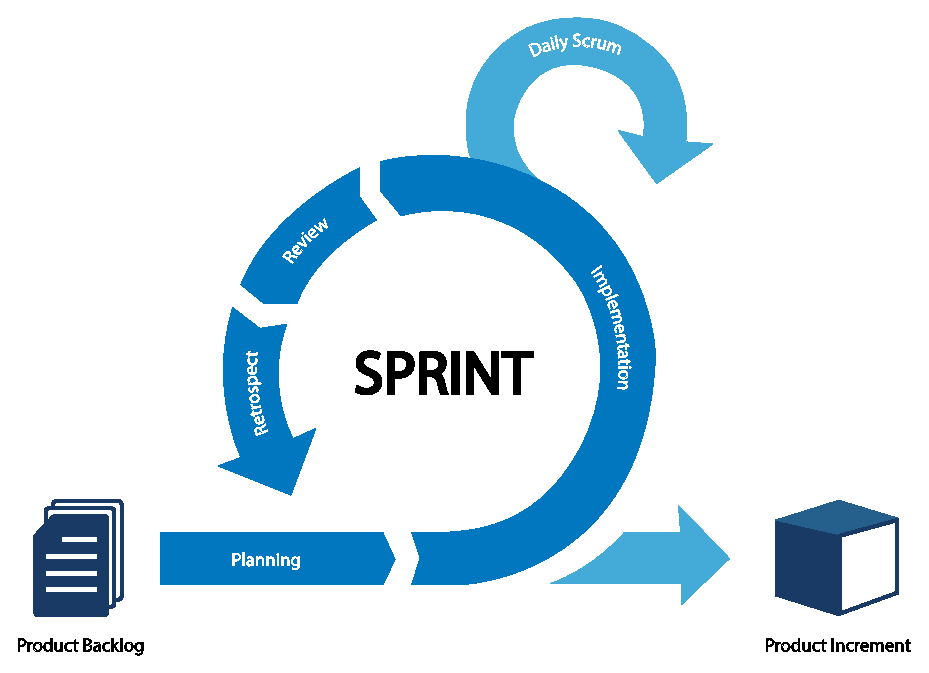
\includegraphics[page=1,width=0.75\textwidth]{sections/theory/figures/scrum.eps}
    \caption{Scrum workflow.}
    \label{fig:scrum}
\end{figure}

\subsection{Kanban}
Kanban~\cite{kanban} is a lean software development methodology, based on the lean methodologies. These have been highly successfully in manufacturing processes. At the center of Kanban is a just-in-time (JIT) process. No new tasks are to be started unless there is a need for it. Further, once a capacity limit has been reached, no further task can be started on. When a task has been resolved, a new one can be started. This can simply be described as a pulling workflow. Kanban also often focuses on the visualization of tasks. This is normally done with a Kanban Board. In contrast to Scrum, Kanban allows for the software to be developed in one large development cycle. It is much more flexible, and does not define any roles.

\section{Git}
Git~\cite{git} is a type of distributed version control system (VCS), originally created by Linus Torvalds in 2005. Git is free and open-source, and is today the most popularly used VCS. It is fast and efficient, able to handle everything from small hobby projects to giant projects like the Linux kernel. Every Git directory is a complete repository with history and full version-tracking abilities. It does not need access to internet, nor a central server in order to work.

\subsection{GitFlow}
GitFlow is a popular branching model for Git, created by Vincent Driessen~\cite{gitflow}. Figure~\ref{fig:gitflow} displays an example git history, adhering to the GitFlow branching style. GitFlow truly excels in parallel development. It is extremely well suited for collaboration and scales well. It also provide an efficient and predictable merging flow, making it easy to customize workflows for various needs.

Development of new features are done in \textbf{feature branches}. These branch off from the \textbf{development branch}, often named \textbf{develop}, reflecting the current state of "development". When a feature is done, it is merged back into the \textbf{development branch}. When it is time for a new release, a \textbf{release branch} is created based on the \textbf{development branch}. In this branch, finishing touches can be made, like bumping up the version numbers, etc. When approved, the \textbf{release branch} is then merged into a \textbf{master branch}, and also back into the \textbf{development branch}. The \textbf{master branch} only contains released code. In the event of an emergency, a \textbf{hotfix branch} can be used. This provides a shortcut for implementing critical fixes. A \textbf{hotfix branch} branches directly from master. When finished, the \textbf{hotfix} is merged into both \textbf{master} and \textbf{develop}.

\begin{figure}[h]
    \centering
    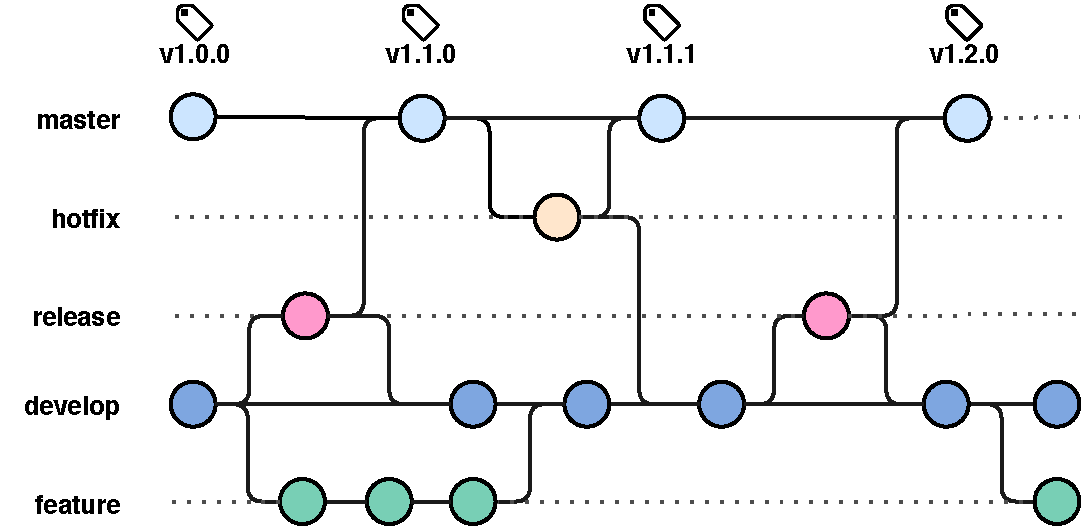
\includegraphics[page=1,width=\textwidth]{sections/theory/figures/gitflow.pdf}
    \caption{GitFlow branching model example.}
    \label{fig:gitflow}
\end{figure}

\section{GitHub}
GitHub is primarily a hosting service for Git repositories. The company was acquired by Microsoft in 2019. In addition to repository hosting, GitHub provides a range of different services through it's web-based GUI. This includes both wikis, access controls, simple task management tools, statistics, automation capabilities and websites hosting.

\subsection{GitHub Actions}
\label{sec:theory-github-actions}
GitHub Actions~\cite{github-actions} is a fairly very new service provided by GitHub. It enables users to automate software workflows, effectively providing a high quality CI/CD for free~\footnote{GitHub Actions usage is completely free for public repositories. For private repositories, depending on the subscription plan, some thousand minutes of free usage is provided each month.}. It is also possible to set up self-hosted runners. GitHub Actions makes it possible to both build, test and deploy code directly from within GitHub.

To setup and configure an automated process, so-called workflows needs to be defined. These are made up of one or more jobs. The actual workflow has to be defined in a YAML file. This file needs to be created and placed in a repository hosted on GitHub. Consult the documentation available at GitHub for the appropriate workflow syntax for creating such YAML files~\cite{github-actions-workflow-syntax}.

\subsection{GitHub Pages}
Github provides its users with a public webpage hosting service. This is named GitHub Pages \cite{github-pages}. User are able to serve static websites directly from their repository hosted on GitHub. Normally, a GitHub Pages site is published by pushing static files to a specific branch named \textit{gh-pages}.

\section{HyperText Markup Language (HTML)}
HTML is a markup language, originally defined by Tim Berners-Lee and Robert Caillau in 1989. It is primarily used for documents on the web, intended to be displayed in a web-browser. It is used for structuring and formatting information. HTML can be used in conjunction with other web technologies such as Cascading Style Sheets (CSS) and scripting languages like JavaScript, in order to either style, or dynamically change and alter the contents of a web page. The currently latest release of the language is HTML5.

\section{Cascading Style Sheets (CSS)}
CSS is short for Cascading Style Sheets. CSS is a programming language in order to describe how HTML elements in a HTML file are to be rendered. Everything from the boldness of a headline, to the background of the entire page.

\section{JavaScript}
JavaScript is a lightweight interpreted programming language. The language is prototype-based, a type of object-oriented programming where properties and methods are added to an instance of an implicitly defined class~\cite{prototype-based-programming}. JavaScript does not provide any type-checking.

JavaScript was developed by Brendan Eichand and released in 1995~\cite{javascript-original-release}. Initially, it was designed to be a small scripting language for enabling interaction with web pages. A standardization effort of JavaScript, led by Ecma International~\cite{ecma-international}, lead to the ECMAScript specification that the modern JavaScript language conforms to. Since then, the language has evolved rapidly and gained massive in popularity. It has become the de-facto language for adding dynamic behavior to HTML. As of may 2020, JavaScript is among the top ten programming languages according to the TIOBE index \cite{tiobe-index}.

% Node.js
Originally, JavaScript engines were mainly used in browser environments. However, with the development of Node.js in early 2009, this was dramatically changed. Node.js provides a runtime environment for executing JavaScript outside of a web browser. It set the stage for server-side JavaScript programs. In January 2010, a package manager named npm \cite{npm} was released for Node.js. This made it easy for developers to share and reuse source code.

% Module bundlers
The size of JavaScript programs has increased massively in size. With increased size, so does the complexity of the code. However, JavaScript had very limited functionality in terms of splitting a program up in smaller modules for use with the browser. Maintaining large codebases was a nightmare. It therefore became apparent that a way of breaking down a JavaScript program into smaller modules was needed. Several open-source module systems were therefore developed by the community in order to tackle this problem.

\subsection{Module systems}
\label{sec:theory-module-system}
\begin{itemize}
    \item \textbf{CommonJS} is a module specification meant for JavaScript outside the browser. It is mainly used in Node.js, and hence it is one of the most popularly used module definitions. The modules are mainly imported and exported with the keywords "require" and "module.exports".
    \item \textbf{Asynchronous module definition}, or more commonly known as AMD, is a JavaScript module definition intended for the browser. It defines an API for defining code as modules, including their dependencies. AMD also has the capability of loading modules asynchronously. The most popular AMD module loader is named RequireJS \cite{requirejs}.
    \item \textbf{Universal Module Definition}, abbreviated UMD, is a module definition wrapper to be able to use various module systems \cite{universal-module-definition}. Be it in the browser or in Node.js. It is compatible with both CommonJS and AMD.
    \item \textbf{JavaScript modules}, or ES Modules, are a language native module system, introduced with ECMAScript 2015 (ES6) in 2015. The implementation is relatively new, so a lot of libraries, frameworks and packages does not support this yet. Still, most browsers have already implemented support for this \cite{es-modules-support}.
\end{itemize}

\subsection{Transpilation}
\label{sec:theory-transpilation}
Due to the many versions of JavaScript, or more specifically ECMAScript, like ES5, ES6 and ES7, compatibility is an issue. Not all browsers and environments support the latest ECMAScript versions. Tools like Babel \cite{babel} has been developed in order to transpile JavaScript to a specific version. The most common transpilation target, supported by all the major browsers is ECMAScript 5 (ES5).

\subsection{Bundling}
\label{sec:theory-bundling}
JavaScript bundling is an optimization technique to combine separate resource files into one file. This is done in order to reduce the number of HTTP requests required for a page to load. Several bundlers are able to do so called tree-shaking, dramatically reducing the size of the finished bundle. In addition to the performance gain, bundling is also often done in order to develop a JavaScript application in separate files, effectively employing a form of module system. The bundlers often use one or more of the popular module systems like UMD and ES modules. There are three main actors in terms of bundling JavaScript.
\begin{itemize}
    \item \textbf{Webpack} \cite{webpack} is a module bundler for JavaScript. However, it is also able to transform front-end assets like HTML, CSS, and images. Webpack is mostly used for bundling JS applications, and is highly extendible. It also provides a way to bundle an application for Node.js to be used in the Browser \footnote{This requires that no Node.js specific APIs are used. Alternatively, polyfills could be supplied.}. However, as of may 2020, it does not support exporting ES Modules.
    \item \textbf{Rollup} \cite{rollup} is a module bundler primarily focusing on JavaScript libraries. It has a lot of similarities with Webpack. However, it is a bit lighter and provides exporting support for ES Modules.
    \item \textbf{Browserify} \cite{browserify} is a lightweight module bundler for enabling the use of CommonJS syntax in the Browser.
\end{itemize}

\section{TypeScript}
TypeScript \cite{typescript} is a typed superset of JavaScript that compiles to plain JavaScript. It is open source, and primarily developed and maintained by Microsoft \cite{microsoft}. TypeScript provides optional static typing to the JavaScript language. The TypeScript compile also includes support for the latest ECMAScript features.

\section{JavaScript Object Notation (JSON)}
JavaScript Object Notation, better known as JSON, is a lightweight data interchange format. It is easy for both humans and machines to read and write. The data is stored as attribute–value pairs. An example is shown in Program Code \ref{lst:json-example}.
\lstinputlisting[language=JSON,style=numbers,caption={Example JSON data},label={lst:json-example}]{sections/theory/code/json-example.json}

\section{JSDoc}
JSDoc is markup language for annotating JavaScript source code files. The JSDoc specification was released in 1999. Today it has become the de-facto JavaScript documentation language. It is for example used in projects like the Google Closure Compiler \cite{google-closure-compiler} by Google. Since JavaScript has no type-checking, JSDoc is able to patch some of this inconvenience. Figure \ref{lst:jsdoc-example} shows an example of JSDoc code, describing a soda bottle class implementation. By using various tools, one is able to generate documentation in formats like HTML and RTF. JSDoc 3 is the current version of the original companion documentation generation tool for JSDoc. JSDoc 3 \cite{jsdoc-3}, also referred to as just JSDoc, is the most used tool for programmatically generating JavaScript documentation. It has a wast feature set, even allowing users to create customized themes, known as templates. Currently, JSDoc is used by more than 38.800 public projects \cite{jsdoc-used-by}, and has over 10.600 stars on GitHub \cite{jsdoc-stargazers}.

\lstinputlisting[language=JavaScript,style=numbers,caption={JSDoc example code},label={lst:jsdoc-example}]{sections/theory/code/jsdoc-example.js}


\section{Tools and libraries}
\subsection{WebGL}
WebGL (Web Graphics Library) \cite{webgl} is a JavaScript API for rendering interactive high-performance 3D and 2D graphics in a web browser. WebGL uses OpenGl ES \cite{opengl-es}, a subset of OpenGL. WebGL makes it possible to take advantage of hardware graphics acceleration provided by the user's device. For actually displaying the graphics in the browser, HTML5 <canvas> elements are used. 

\subsection{three.js}
three.js\cite{three.js} is a cross-browser JavaScript library for creating and displaying 3D computer graphics in a web browser. It is open-source and licensed under the MIT license. three.js uses WebGL under the hood. The library abstracts away a lot of tedious manual labour, like the setup of WebGL, construction of vertices, faces, etc. three.js provides the user with an easy API for directly constructing three-dimensional objects like boxes, spheres and toruses, as well as easy camera controls. The library also includes a vast set of shaders, making it very simple to make use of high quality materials. three.js is one of the most popular 3D graphics JavaScript library for use in the browser, as can be seen on its GitHub repo \cite{three.js}.

\subsection{ndarray}
\label{sec:theory-ndarray}
ndarray is an open-source JavaScript package providing modular multidimensional arrays, written by Mikola Lysenko in 2013. In short, ndarray implement a higher dimensional views of 1D arrays. The 1D array can either be a normal JavaScript Array, or a JavaScript typed array. MDN defines typed arrays as \textquote[\citet{mdn-typed-arrays}]{array-like objects that provide a mechanism for reading and writing raw binary data in memory buffers.}. Mainly, they are used for maximizing efficiency and reducing memory footprint. However, typed arrays are normally quite difficult to work with in JavaScript. Multidimensional typed arrays even more so. ndarray provides a simple but powerful API, making use of multidimensional typed arrays easy.
\colorbox{red}{strided arrays??}

\subsection{Electron}
Electron \cite{electron} is an open-source framework developed and maintained by \citet{github}. It allows one to build cross-platform desktop applications with JavaScript, HTML and CSS. Electron is used by thousands of people, and apps like Visual Studio Code \cite{visual-studio-code}, Facebook Messenger \cite{messenger} and Microsoft Teams \cite{teams} are all made with Electron.

\subsection{React}
React \cite{react} is a JavaScript library for building user interfaces, created by \citet{facebook}. It is based around components, where each component manage its own state. These are then composed together, enabling the creation of intricate and complex UIs. The library also implements its own syntax extension to JavaScript. It is named JavaScript XML, or the more popular used term - JSX. In addition to this, there exists a vast ecosystem of plugins for React, greatly simplifying the implementation of everything from localization to state management.

\subsection{Semmle LGTM}
\label{sec:theory-semmle-lgtm}
LGTM by Semmle \cite{lgtm} is a web service providing code security analysis. The service is free for open-source projects. LGTM integrates with sites like GitHub and Bitbucket, and is able to analyze projects written in Java, Python, JavaScript, TypeScript, C\#, Go, C and C++. It seeks out to combat the manual process of finding vulnerabilities. By catching them at an early stage, one can prevent vulnerabilities from reaching production. LGTM is based on large community of top security researchers, making it possible to help developers ship secure code \cite{lgtm-security}.

\subsection{Coveralls}
\label{sec:theory-coveralls}
Coveralls \cite{coveralls} is a web service for code testing coverage. It enables one to track a projects code coverage over time, providing valuable insight in a projects testing suite. Coveralls also features close integration with GitHub, enabling pull request coverage reviews.

\section{3D computer graphics}
3D computer graphics refers to three-dimensional representation of geometric data in computers, normally to be rendered into a two-dimensional image. The finalized render may be saved or displayed on a screen in realtime. The geometric data is usually a 3D model, stored in an appropriate file format. The most basic polygon primitives in computer graphics includes vertices, edges and faces. A vertex is simply point in space. An edge is a connection between two vertices. A face is a closed set of edges. Figure \ref{fig:triangular-mesh} shows a yellow triangle with the appropriate vertex, edge and face labels. These primitives together defines a polyhedral. Polyhedrons can then be further grouped together into a mesh. The most common type of polygon mesh is a triangular mesh. This is a mesh comprised of only triangles. Figure \ref{fig:triangular-mesh} shows an illustration of a section of a triangular mesh.
\begin{figure}[h]
    \centering
    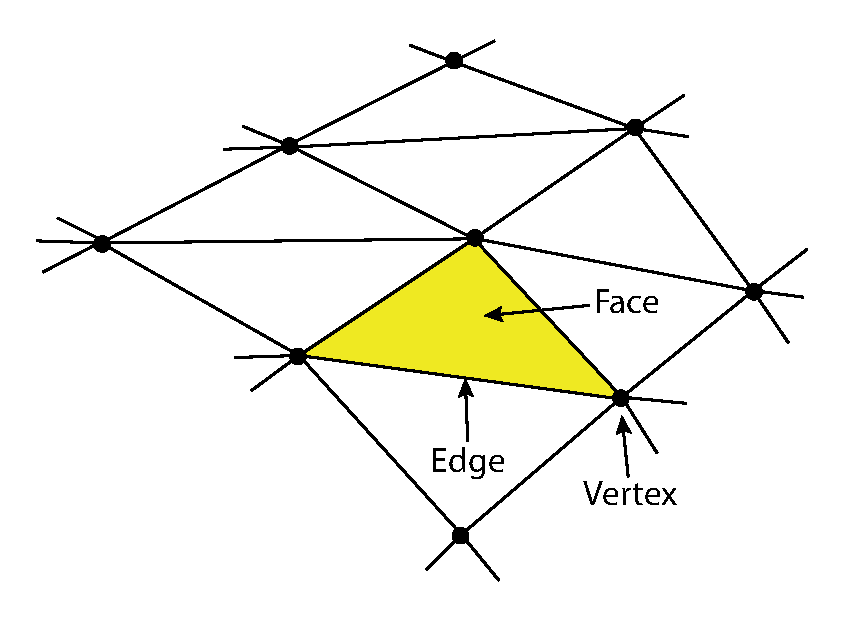
\includegraphics[width=0.75\textwidth]{sections/theory/figures/mesh.eps}
    \caption{Triangular mesh}
    \label{fig:triangular-mesh}
\end{figure}

\subsection{Texture maps}
\label{sec:info-texture-maps}
A texture map is an image which is applied, or mapped, onto the surface of a geometry. The images is often in the form of a bitmap image or a procedural texture. Texture mapping, or UV mapping, is the process of projecting an actual 2D image onto a 3D model. The technique was initially developed by Edwin Catmull in 1974 \cite{catmull-texture-mapping}. UVs are two-dimensional texture coordinates, assigned to every vertex in a polygon. They are essential in terms of describing how an image gets applied onto a geometry. Figure \ref{fig:texture-mapping} shows an illustrative example of how a 2D image gets "wrapped" around a 3D model. A lot of 3D modeling software are able to do the UV unwrapping automatically, for example Blender \cite{blender}. It is also possible to map a finalized render into a surface texture, a process known as baking \cite{blender-texture-baking}. This is primarily used as an optimization technique.

\begin{figure}[h]
    \centering
    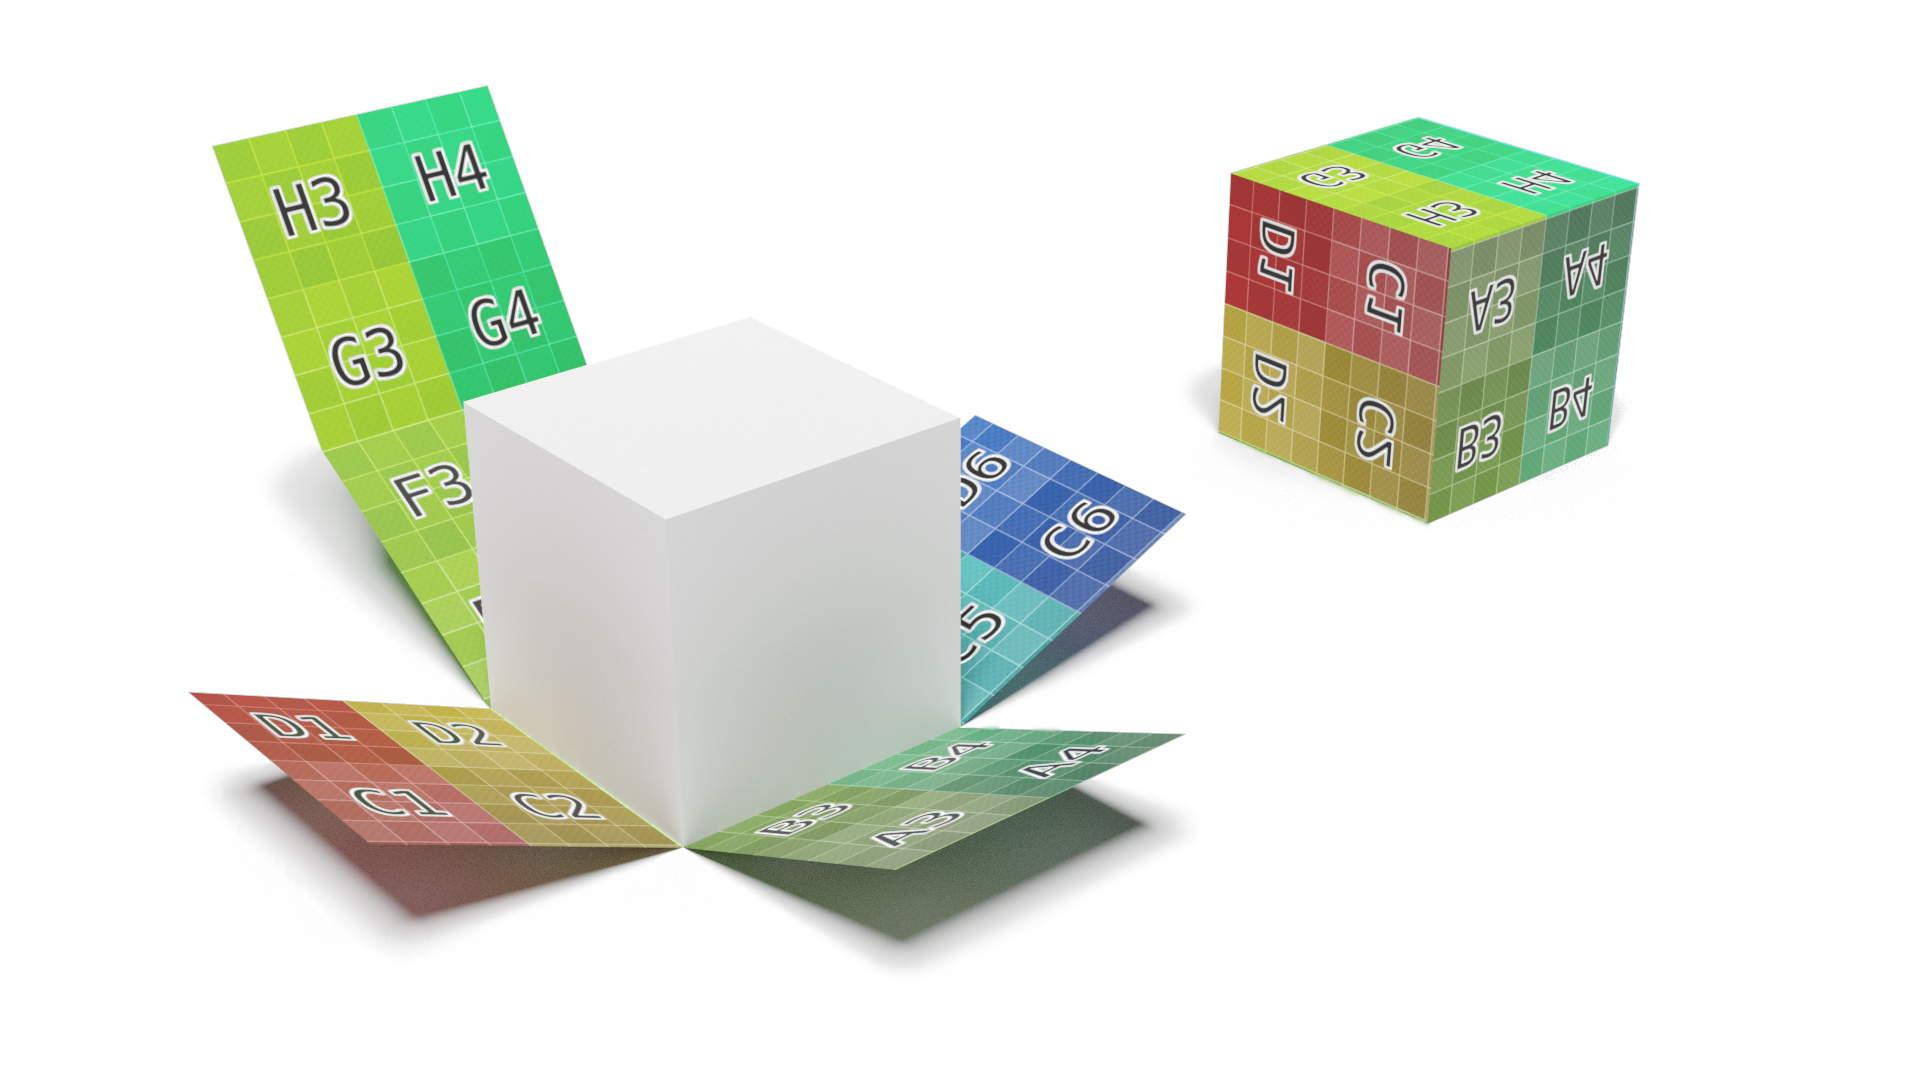
\includegraphics[width=\textwidth]{sections/theory/figures/texture-mapping.png}
    \caption{Texture mapping illustration.}
    \label{fig:texture-mapping}
\end{figure}

\subsection{Ray casting}
\label{sec:theory-raycasting}
Ray casting is the concept of use of ray–surface intersection tests to solve a variety of problems in 3D computer graphics and computational geometry. 
The first use of the term ray casting was made by Scott Roth, in a paper from 1982 titled "Ray casting for modeling solids" \cite{roth-ray-casting}. Raycasting is demonstrated in Figure \ref{fig:raycasting-intersections-example}. A ray is directed towards an object. If it crosses a face, an intersection is registered.

\begin{figure}[h]
    \centering
    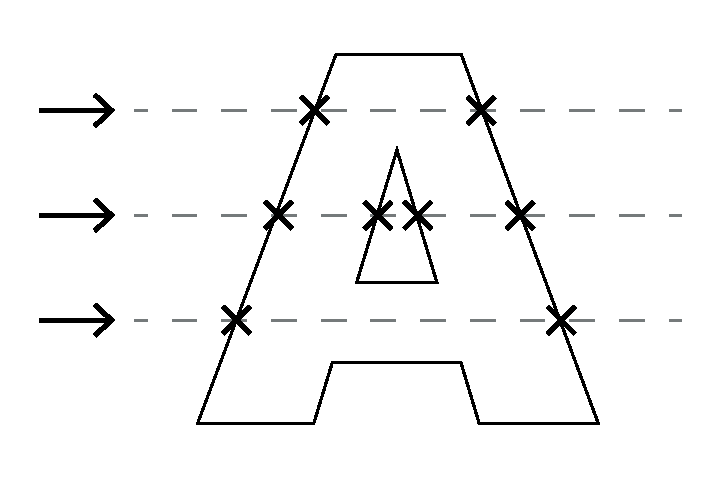
\includegraphics[scale=0.8]{sections/theory/figures/raycast-intersections}
    \caption{Raycasting intersections example.}
    \label{fig:raycasting-intersections-example}
\end{figure}

\section{Acceleration data structures}
\subsection{Octrees}
\label{sec:theory-octree}
An octree is a type of tree structure. Each internal node of an octree has exactly eight children. An octree is most commonly used for partitioning three-dimensional space. This is done by recursively subdividing the space into eight octants. Note that depending on the number of recursive subdivisions, an octree may contain multiple objects in its leaf nodes. Figure \ref{fig:octree-example} shows an example of an octree with three levels. Octrees are very commonly used in 3D computer graphics. Another common use case of octrees is for storing voxel data. 

\begin{figure}[ht]
    \centering
    \begin{subfigure}[c]{0.33\textwidth}
        \vspace{0pt}
        \centering
        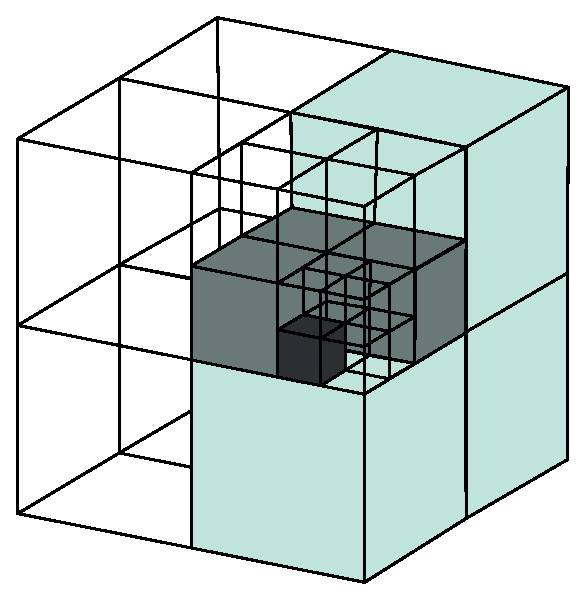
\includegraphics[width=\textwidth]{sections/theory/figures/octree-cube.eps}
    \end{subfigure}
    \hspace{1cm}
    \begin{subfigure}[c]{0.5\textwidth}
        \vspace{0pt}
        \centering
        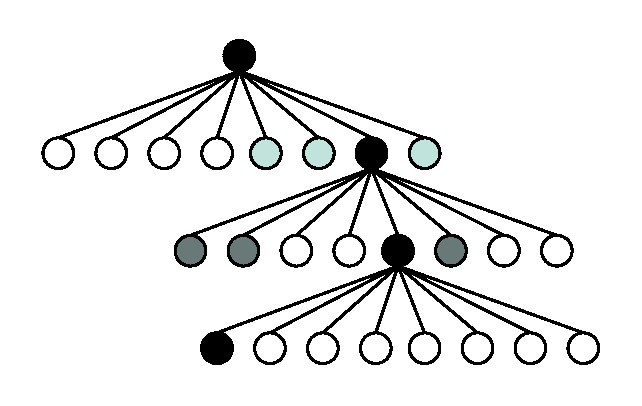
\includegraphics[width=\textwidth]{sections/theory/figures/octree-tree.eps}
    \end{subfigure}
    \caption{Example of an octree with three levels.}
    \label{fig:octree-example}
\end{figure}

\subsection{Bounding volume hierarchy }
A bounding volume hierarchy, abbreviated BVH, is a tree structure on a set of geometric objects. A BVH construction algorithm partitions the actual objects. The objects are wrapped in a so-called bounding volume, forming the leaves of the tree. These are then grouped together into a larger bounding volume. This process is then repeated in a recursive manner. The result is a tree structure with one single bounding volume as the root node. An example of a BVH is shown in Figure \ref{fig:bvh-example}. BVH are often used for accelerating collision detection and raytracing.

\begin{figure}[ht]
    \centering
    \begin{subfigure}[c]{0.37\textwidth}
        \vspace{0pt}
        \centering
        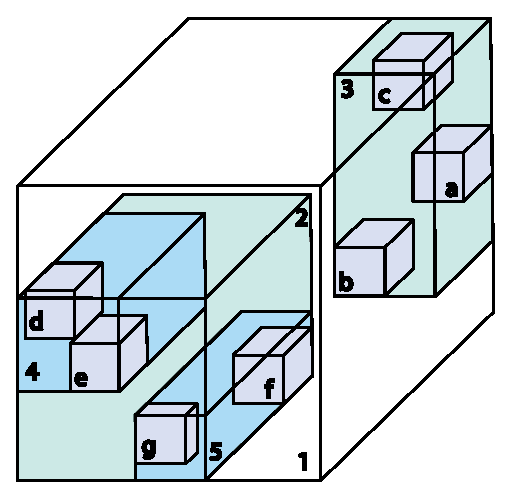
\includegraphics[width=\textwidth]{sections/theory/figures/bvh-cube.eps}
    \end{subfigure}
    \hspace{1cm}
    \begin{subfigure}[c]{0.45\textwidth}
        \vspace{0pt}
        \centering
        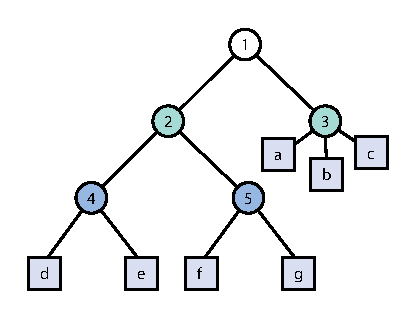
\includegraphics[width=\textwidth]{sections/theory/figures/bvh-tree.eps}
    \end{subfigure}
    \caption{Example of an BVH. Replica of figure from \citet{mcdonald1988}.}
    \label{fig:bvh-example}
\end{figure}

\section{Voxel}
A voxel is the three-dimensional analogue of a pixel \cite{wiki-voxel}. It represents a single data point in a regularly spaced three-dimensional grid. Figure \ref{fig:three-voxels} shows an illustration of three voxels, where one of the voxels are marked with blue color. A very common use of voxels are in medical imaging, for example datasets produced by a CT scan. Other areas where voxels are commonly used includes simulations and for representing terrain in games.

\begin{figure}[h]
    \centering
    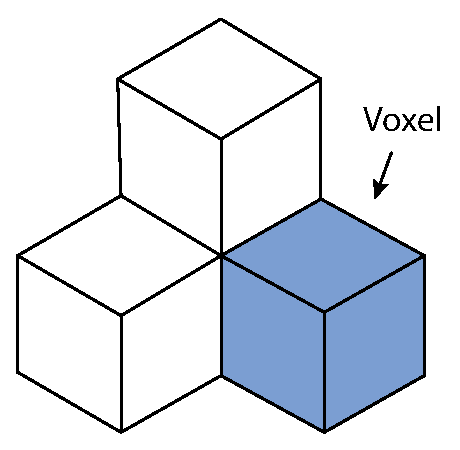
\includegraphics[width=0.4\textwidth]{sections/theory/figures/voxels.eps}
    \caption{Three voxels.}
    \label{fig:three-voxels}
\end{figure}

\section{Voxelizer v0.1.3}
\label{sec:voxelizer-v013}
Voxelizer v0.1.3 \cite{voxelizer-v0.1.3} is a JavaScript engine (or library) for conducting voxelization of 3D models. It was written by me, André Storhaug, in 2019. Version 0.1.3 features a relatively simple voxelization algorithm which is based on raycasting. The sampling algorithm tries to produce a filled volume-representation of a supplied 3D model. It samples the front and the back of the model, combines the two results together and tries to fill the in-between gap. The 3D model loading capabilities of the program is limited to plain OBJ files. In terms of exporting, the software is able to output a 3D JavaScript array (nested arrays).

The engine is using ES6 features, hence it is transpiled with Babel (see Section \ref{sec:theory-transpilation}). However, is not bundled. It is therefore not possible to use the program out of the box in a browser. One is limited to Node.js, or setting up a build system involving a module bundler like Webpack or Rollup, as described in Section \ref{sec:theory-bundling}. The source code is messy, and it is very hard to extend functionality. Especially due to a severe lack of documentation.

Voxelizer v0.1.3 produces unsatisfactory voxelization results. Firstly, several of the voxelizations contains holes. This can be clearly seen in Figure \ref{fig:voxelizer-v0.1.3-torus}. A voxelization with holes often renders the voxelization useless. Secondly, a lot of artifacts are often generated, severely degrading the results. This is shown in Figure \ref{fig:voxelizer-v0.1.3-monkey}, where long strains of voxels appear in the front of the model. This is especially pronounced around the ears of the monkey. Thirdly, the software is only able to produce a filled voxelization result. This is mainly due to the fact that the model is only sampled from the front and back. The other sides of the model are not taken into account. This means that shell voxelization is not an option, and details may be lost.

\begin{figure}[p]
    \centering
    \begin{subfigure}[b]{0.49\textwidth}
        \centering
        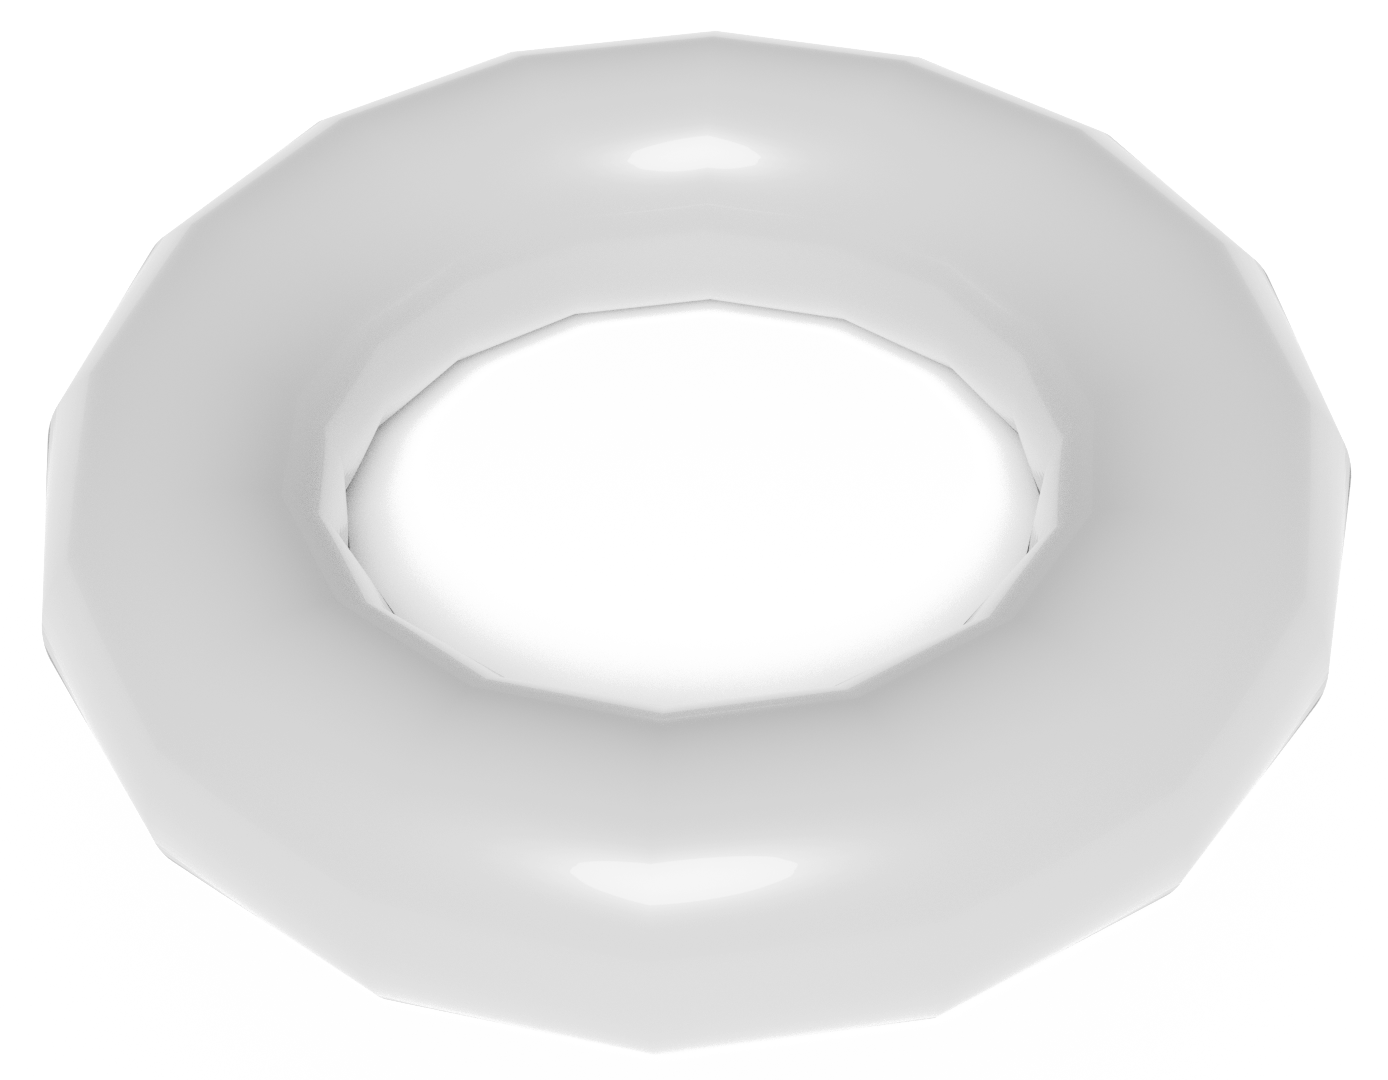
\includegraphics[width=\textwidth]{sections/theory/figures/torus.png}
        \caption{Original torus mesh.}
        \label{fig:original-torus}
    \end{subfigure}
    \hfill
    \begin{subfigure}[b]{0.49\textwidth}
        \centering
        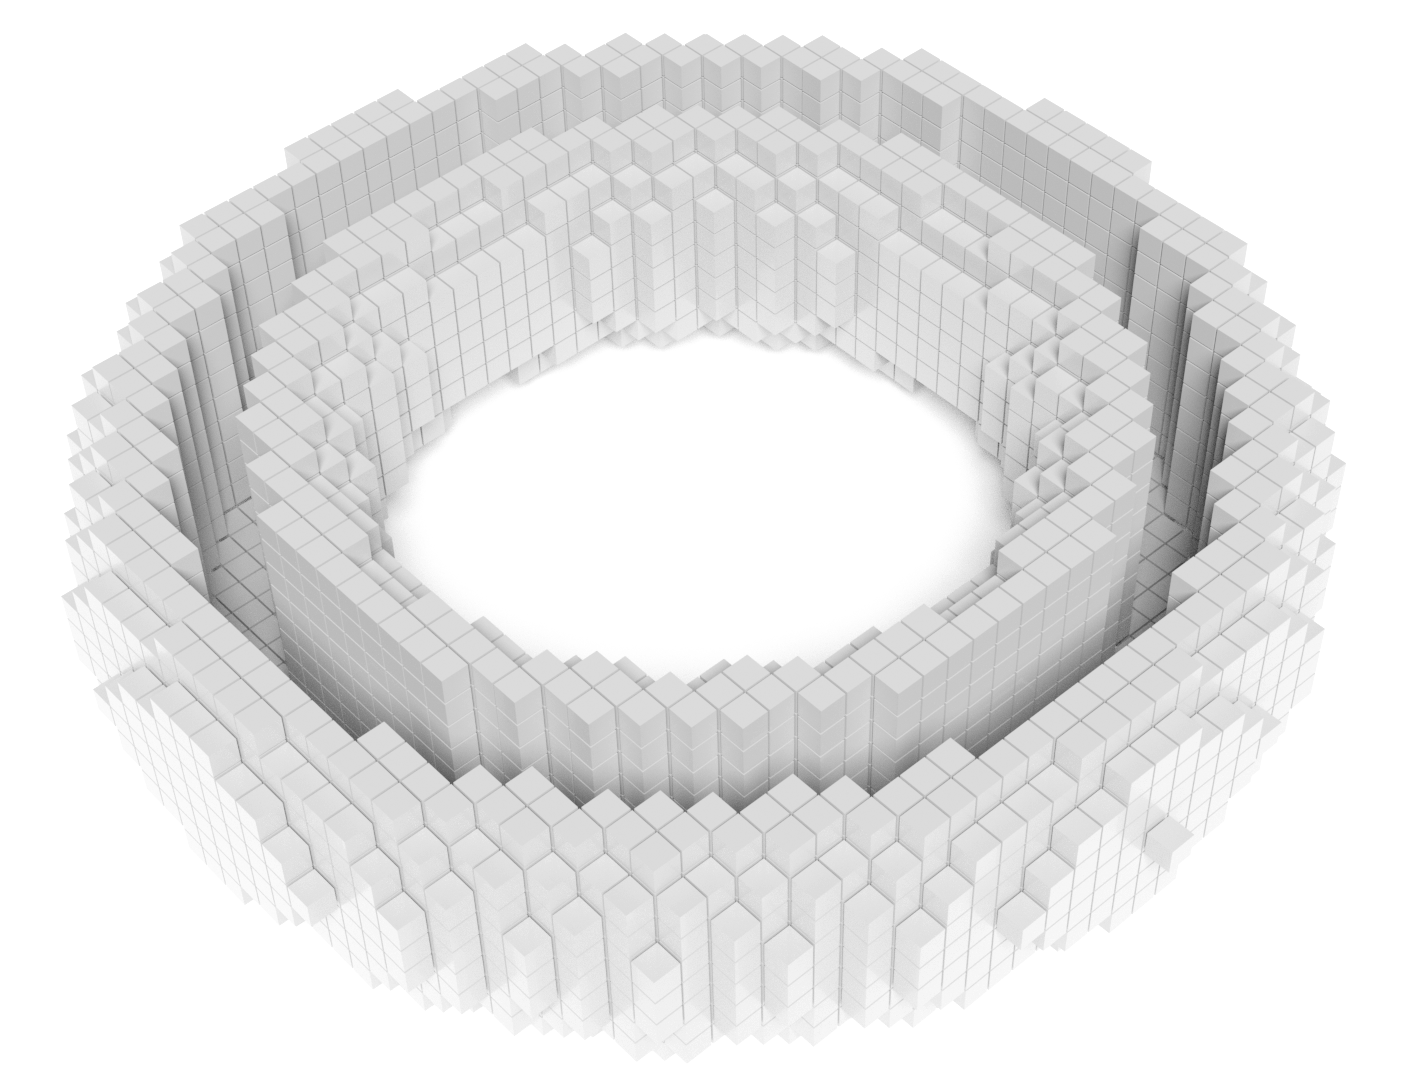
\includegraphics[width=\textwidth]{sections/theory/figures/voxelizer-v013-torus-40.png}
        \caption{Voxelized result.}
        \label{fig:voxelizer-v0.1.3-torus}
    \end{subfigure}
    \caption{Voxelization of a torus with Voxelizer v0.1.3. The voxelization is done with a resolution of 40.}
    \label{fig:voxelizer-v0.1.3-torus}
\end{figure}

\begin{figure}[p]
    \centering
    \begin{subfigure}[b]{0.46\textwidth}
        \centering
        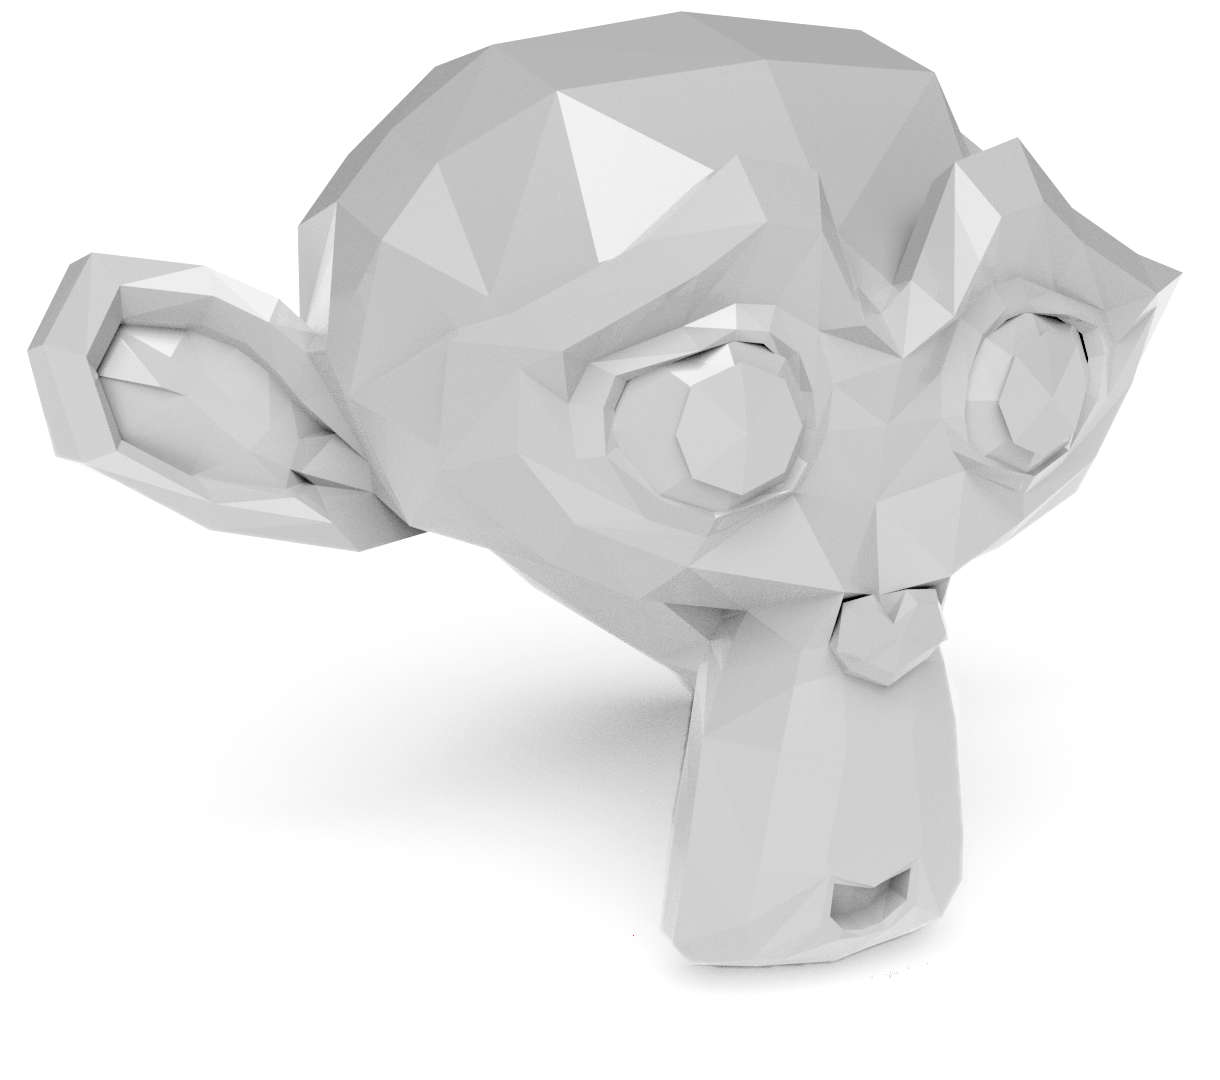
\includegraphics[width=\textwidth]{sections/theory/figures/monkey.png}
        \caption{Original monkey mesh.}
        \label{fig:original-monkey}
    \end{subfigure}
    \hfill
    \begin{subfigure}[b]{0.53\textwidth}
        \centering
        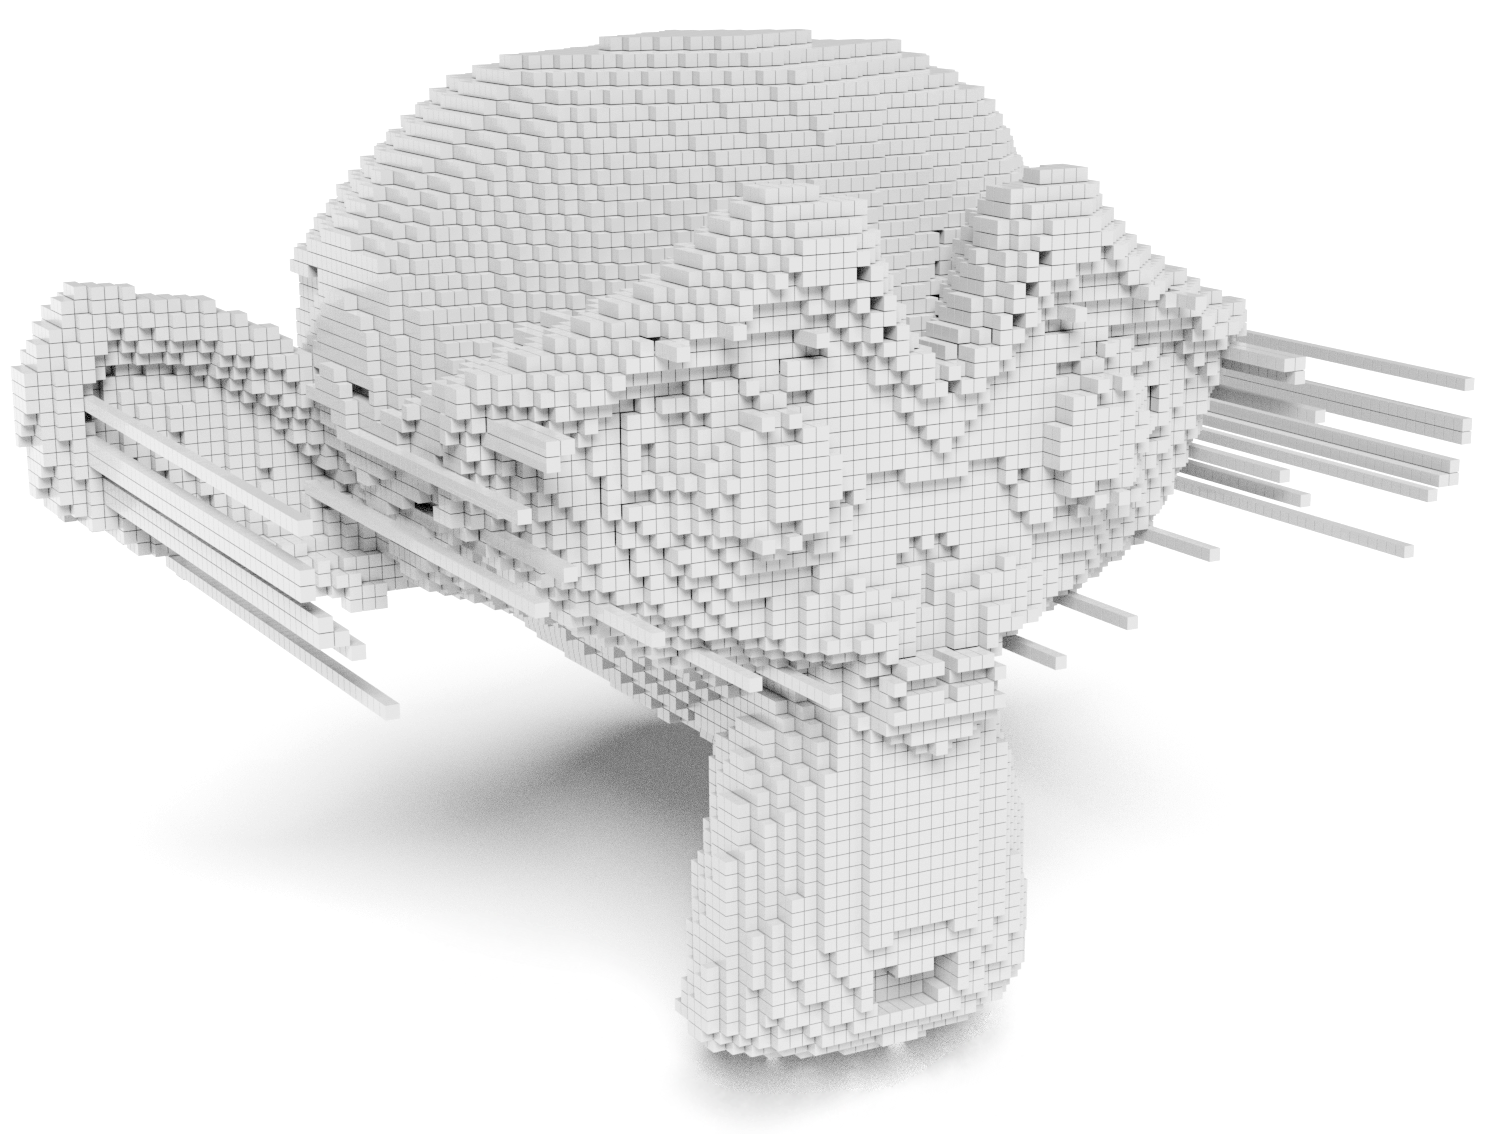
\includegraphics[width=\textwidth]{sections/theory/figures/voxelizer-v013-monkey-100.png}
        \caption{Voxelized result.}
        \label{fig:voxelizer-v0.1.3-monkey}
    \end{subfigure}
    \caption{Voxelization of a monkey with Voxelizer v0.1.3. The voxelization is done with a resolution of 100.}
    \label{fig:voxelizer-v0.1.3-monkey}
\end{figure}
